\chapter{Robot Firmware Implementation}
\label{chp:robotfwimp}
\lhead{Chapter \ref{chp:robotfwimp}. \emph{Robot Firmware Implementation}}

With the creation of the software embedded Bluetooth stack and the \textit{ExplorerBot} test robot platform hardware, it was necessary to integrate these two components into a functional prototype. By using the Bluetooth stack in a real-world, practical application while it was being developed, the quality, effectiveness and completeness of the stack could be evaluated.

\section{Build Dependencies}

To match the Bluetooth stack, each module was written in the C language, and targeted at the free open source AVR-GCC compiler and avr-libc library. A standard \textit{makefile} included with the firmware allows for command line control over the building of the project files into a set of binaries which can then be programmed into the target microcontroller for use via the command \texttt{make all}. The following tools are required to build the firmware under Windows:

\begin{itemize}
	\item The \textbf{WinAVR 20100101} release download, or Windows binaries of the \textbf{GNU Shell Utilities}
	\item The latest \textbf{AVR Toolchain} release download from Atmel (included with Atmel's free \textit{AVRStudio 5} software)
\end{itemize}

Under Debian Linux environments, the following packages are required:

\begin{itemize}
	\item \textbf{gcc-avr} 
	\item \textbf{binutils-avr}
	\item \textbf{avr-libc}
	\item \textbf{avrdude}
\end{itemize}

Which can be installed via the command prompt using the command \texttt{sudo apt-get install gcc-avr binutils-avr avr-libc avrdude}.

\section{Firmware Overview}

The completed firmware of the \textit{ExplorerBot} prototype was developed in a modular manner, to match the corresponding hardware components. This top-down methodology ensured that each portion of the firmware could be mocked up, tested and integrated as needed. Additionally, separating out the firmware components into logical modules gave the final firmware a level of flexibility which should allow for easy modification to suit any hardware changes made to those of the prototype. The completed set of modules (see Figure \ref{fig:robotblockfw}) served as the complete firmware for the robot.

\begin{figure}[H]
	\vspace{1em}
	\centering
		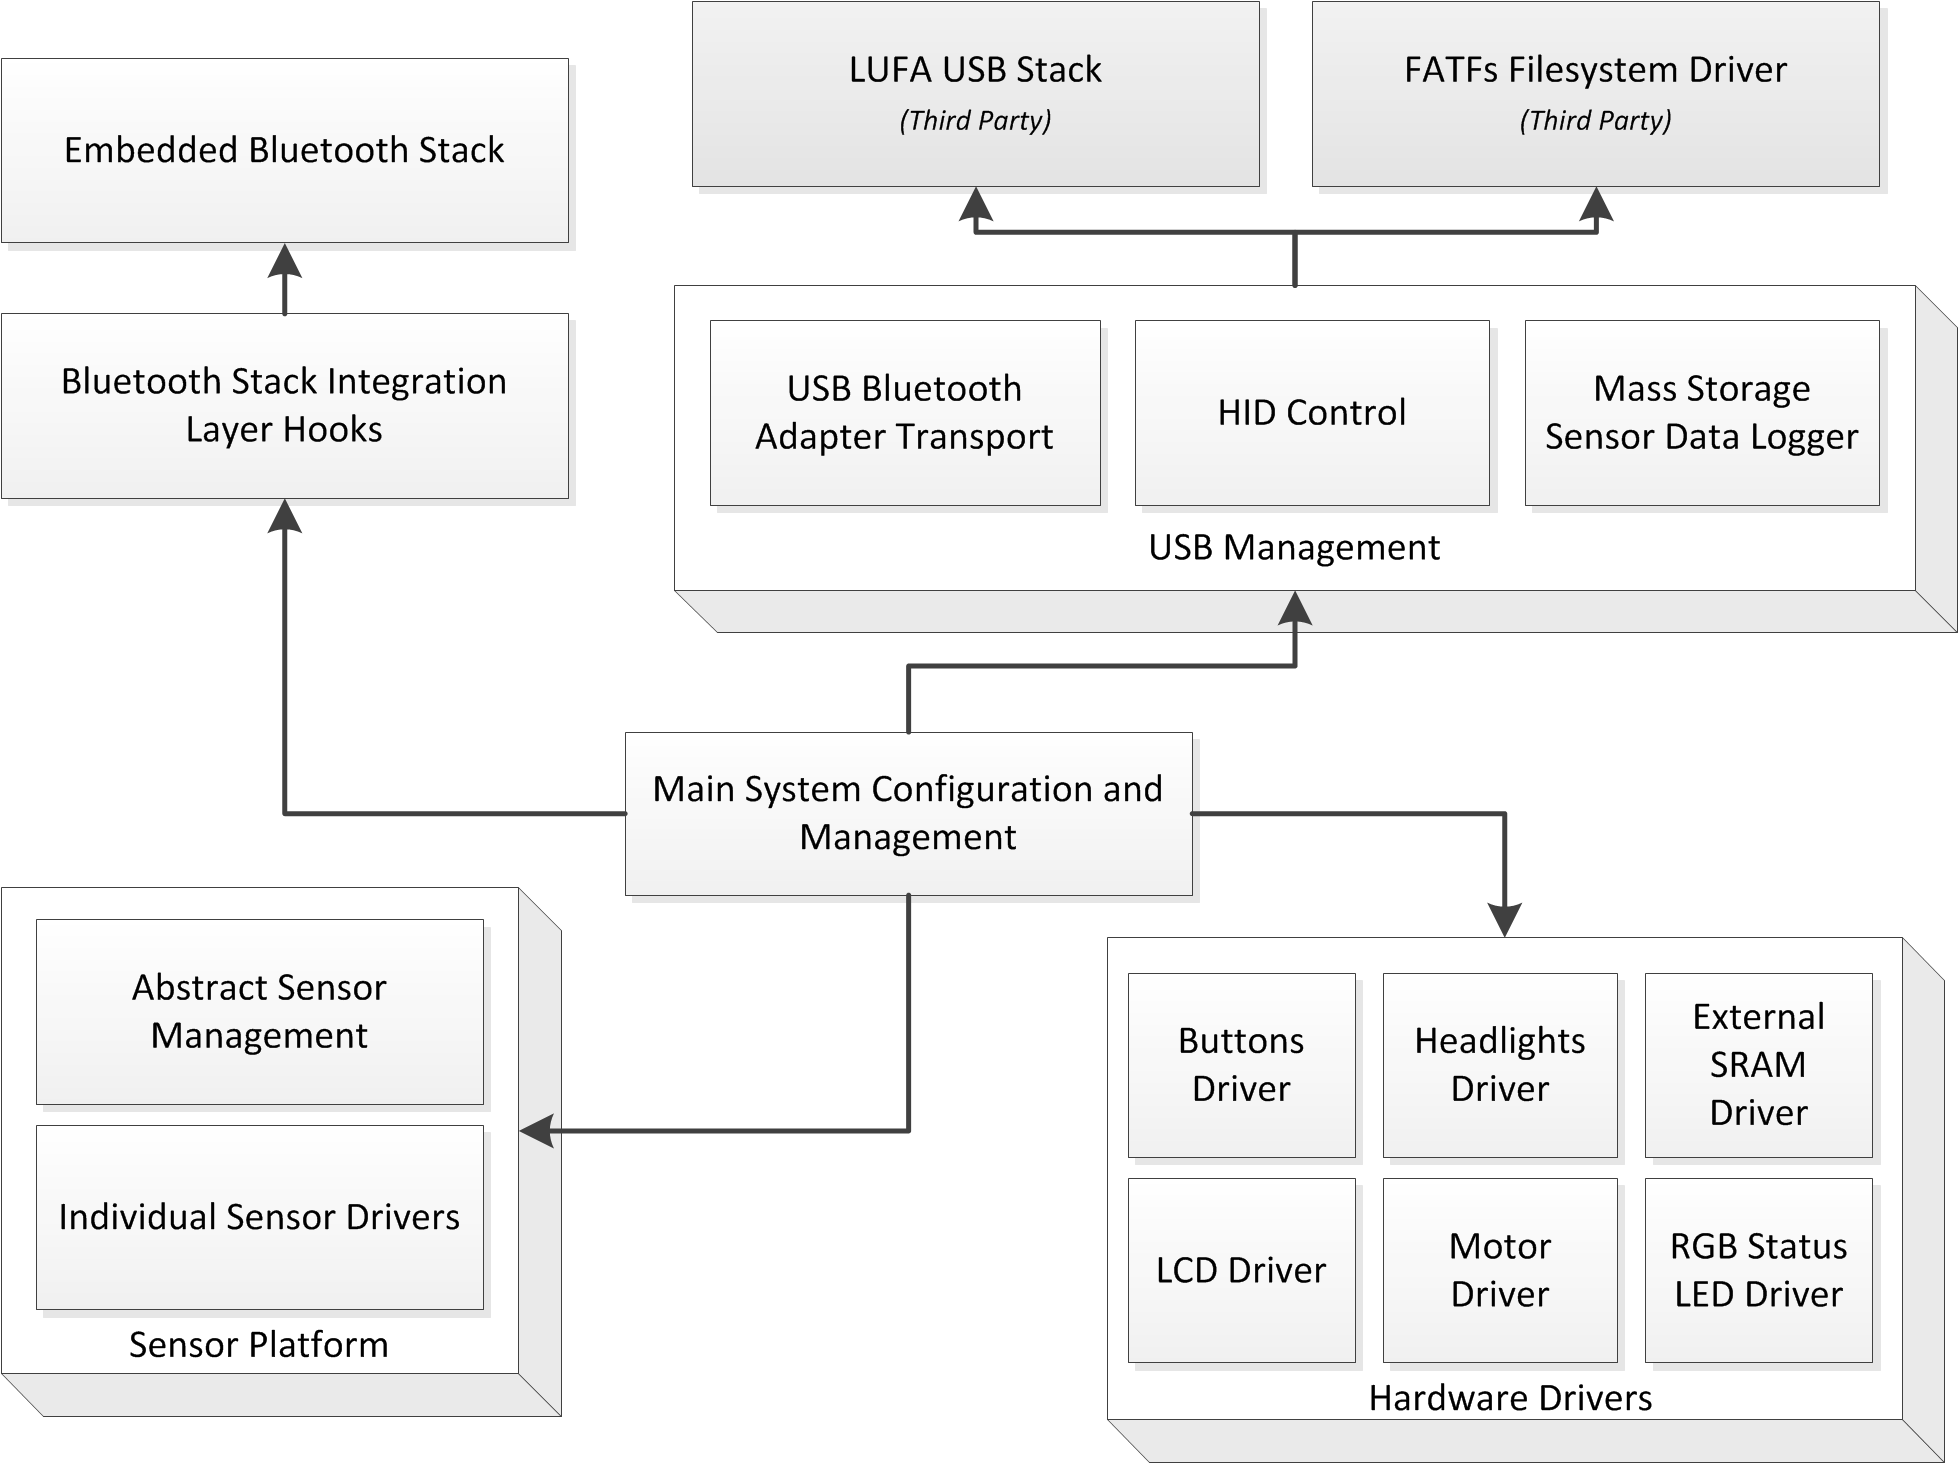
\includegraphics[width=140mm]{FirmwareBlockDiagram.png}
	\rule{35em}{0.5pt}
	\caption[Firmware Block Diagram]{Robot Firmware Block Diagram}
	\label{fig:robotblockfw}
\end{figure}

\section{Firmware Modules}

In this section, each of the robot firmware's main software modules are listed and described in additional detail so that the overall design and implementation of the firmware can be further understood.

\FloatBarrier
\subsection{Main System Control and Configuration}

The main entry point and system loop of the firmware was contained into a single top level module. This module was then made responsible for the initial system hardware configuration, as well as the management of the main loop to dispatch the service task functions in each sub-module.

\FloatBarrier
\subsubsection{System Initialization}

A series of initialization steps are followed during the hardware configuration step; first, the system watchdog (enabled if the chip was last reset through the expiry of the watchdog peripheral's timer) is disabled, the system CPU clock prescaler disabled to ensure the full 16MHz CPU clock speed is used, unused peripherals are powered down and the JTAG debug interface turned off so that the GPIO pins could be used for the RGB status LED. This latter procedure removes the ability to debug the firmware with an external JTAG debugger, however during development it was commented out.

Next, the setup routine calls each hardware driver module's \lstinline{Init()} function, which serves to initialize each hardware module and configure the appropriate hardware ready for use. Finally, one of the robot's remaining 16-bit hardware timers is then configured to run at a 10ms period to serve as the master system tick for timeout management and time based events.

\FloatBarrier
\subsubsection{Start-up Tasks}

Once all the system hardware is initialized, the main program flow then executes the start-up tasks; an informational message is displayed to the LCD while the RGB status LED sequences through all possible combinations, and the sensor platform is initialized to determine which sensors are currently connected. The state of each sensor is then displayed briefly onto the LCD using custom LCD character definitions before the main loop starts (see Figure \ref{fig:sensorinitlcd}).

\begin{figure}[tbph]
	\vspace{1em}
	\centering
		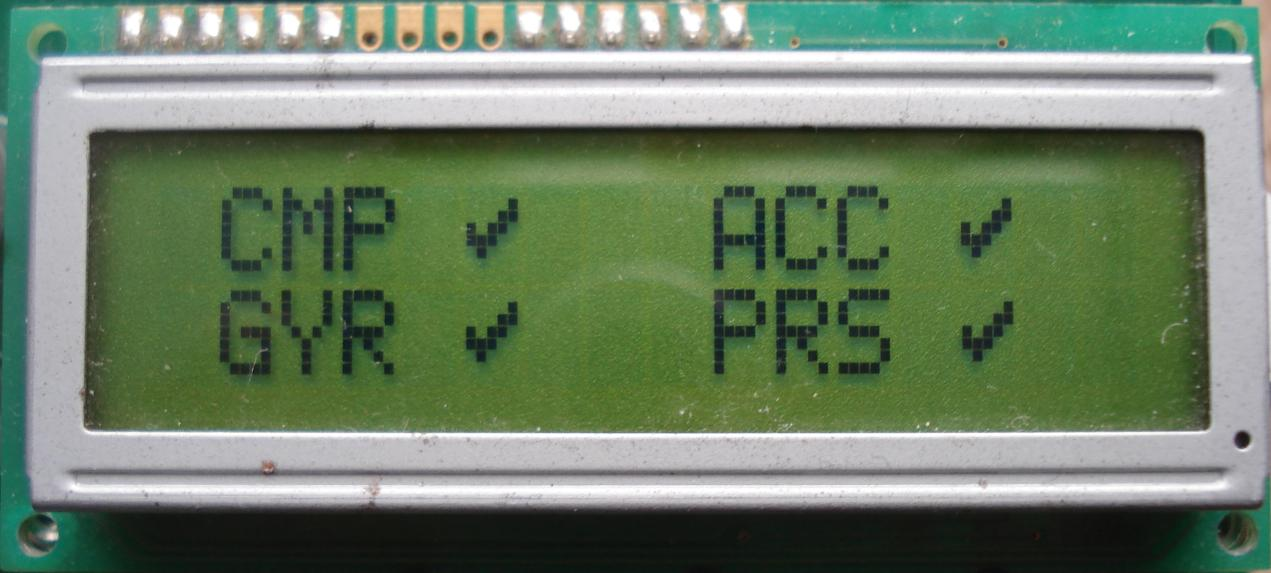
\includegraphics[width=70mm]{LCDSensorsOK.jpg}
		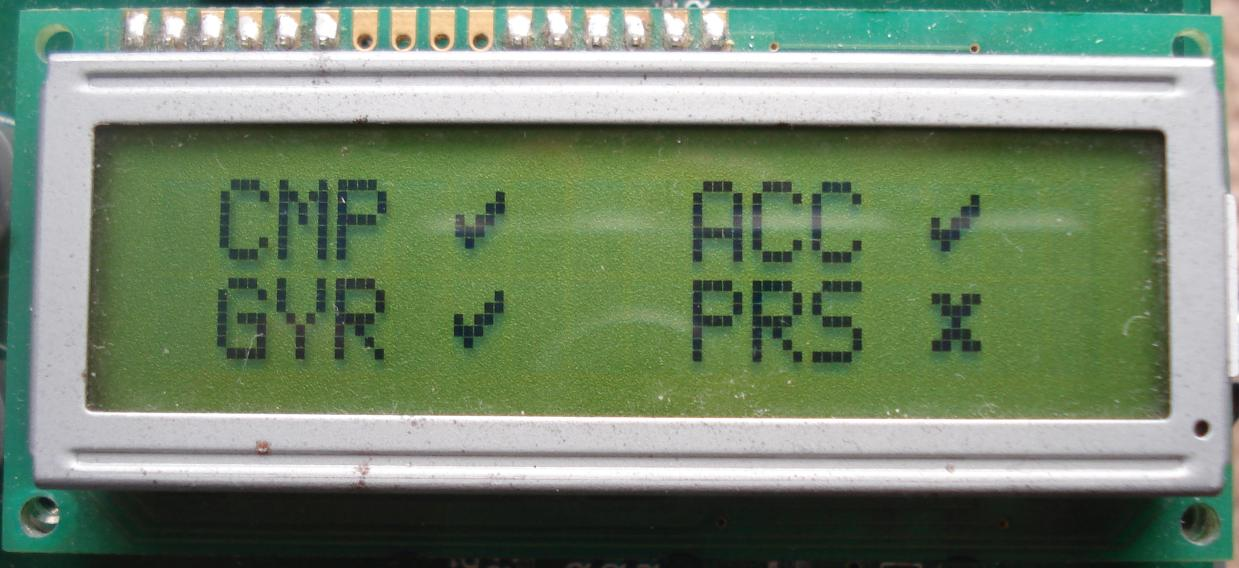
\includegraphics[width=70mm]{LCDSensorsFail.jpg}
	\rule{35em}{0.5pt}
	\caption[LCD Sensor Status Information]{Photos of the LCD display showing successful (\textit{left}) and failed (\textit{right}) initialization.}
	\label{fig:sensorinitlcd}
\end{figure}

\FloatBarrier
\subsubsection{Main Program Loop}

As is the case with virtually all embedded systems, the main program execution was contained in an infinite loop; each iteration of the loop would dispatch to the various sub-components of the system to manage and react to various stimuli. In the case of the robot firmware, the main loop contained three main functions; one, it checked for presses of either of the two physical buttons on the robot, two, it would check for expiry of the system tick timer to dispatch timing-related events, and three, it would execute the various hardware and software module service tasks.

In the case of the two physical buttons, the first (top) button was assigned a soft-reset role, in the case of a communication failure which resulted in the robot's motors being left on and the system uncontrollable. This \textit{emergency stop} style functionality was implemented using the microcontroller's internal watchdog system to reset the microcontroller approximately 15ms after the button press was detected. The second physical button was assigned a mode-specific role, according to Table \ref{tab:buttonroles}.

\begin{table}[tbph]
	\vspace{1em}
	\begin{center}
		\begin{tabular}{ | l | l | }
			\hline
			\textbf{Mode} & \textbf{Function} \\ \hline

			Bluetooth Mode & Initiates a connection to stored Bluetooth device address \\ \hline
			HID Mode & \textit{Unused} \\ \hline
			Mass Storage Mode & Enables sensor logging to the attached flash drive \\ \hline
		\end{tabular}
		\caption[Mode Specific Button Roles]{Table showing the function of the mode-specific physical pushbutton.}
		\label{tab:buttonroles}
	\end{center}
\end{table}

Each time the main loop detected that the system update tick timer period had elapsed, it would notify all timing-dependant hardware modules of this fact; for example, the LCD driver relies on these updates to automatically fade the LCD backlight brightness after a given period of inactivity. Also performed in this section is the update of the sensor values via the sensor platform at regular intervals, and the logging of this data either to the attached Mass Storage USB disk (if logging is enabled) or an established virtual serial connection to a remote PC via Bluetooth.

\FloatBarrier
\subsection{Hardware Drivers}

At the point at which the abstract software in the device needed to interact with the physical board hardware, a set of hardware abstraction drivers was created. These drivers served to encapsulate the functionality of the physical hardware and expose that functionality to the rest of the firmware via a set of basic control API functions. Not every driver sought to expose all the possible abilities of the hardware; due to time constraints only those features actually required by the prototype robot firmware were implemented in most cases.

\FloatBarrier
\subsubsection{Buttons Driver}

The hardware for the board button driver was, as expected, very simple; no debouncing was implemented in the driver itself, as this was not found to be necessary in the firmware. Adequate debouncing for the button logic could be achieved elsewhere in the code instead, via the software flags the buttons controlled.

As a result, the completed button driver implementation was trivial, consisting only of a configuration routine to configure the appropriate GPIO lines as inputs with the microcontroller's internal pull-up resistors enabled, and a status routine to read and mask out the appropriate port lines.

\FloatBarrier
\subsubsection{External SRAM Driver}

While the selected AT90USB1287 microcontroller contained 8KB of SRAM internally for stack, global variables and other working-set data, an external 128KB SRAM IC was mounted externally on the microcontroller board. This memory was attached to the AVR's external memory interface bus, and could then be used to extend the SRAM memory space at the cost of an extra CPU cycle for each external bus access.

Unfortunately, while this external SRAM memory uses a 17-bit address, the AVR's external memory bus interface is only 16-bits wide. As a result, a small software shim driver was required to perform manual bank swapping when required to select one of the two halves of memory. This total 128KB of external SRAM memory was thus divided into two 64KB memory banks, only one of which could be selected at one time.

\FloatBarrier
\subsubsection{Headlights Driver}

Like the button driver, the headlight driver contained only a thin wrapper around the GPIO pin used to control the robot's headlights. Latching of the headlight state was achieved through the GPIO hardware itself; once set to a particular state, the headlights would remain in that state (illuminated or disabled) until changed by a subsequent call to the module's update routine.

\FloatBarrier
\subsubsection{LCD Driver}

The LCD chosen for the robot contained a chipset compatible with the HD44780 display controller, common to many embedded systems where complex graphics are not required. As a result, there is already a plethora of LCD drivers available on the internet from hobbyists and from most microcontroller silicon vendors. Despite this, a simple custom LCD driver was written from scratch for the project, to ensure that as much of the project as was practical remained under the sole author's copyright and distribution control.

While the robot hardware contained a direct hardware connection to the LCD display's \textit{R/W} pin (for read/write control) the final driver code used a more basic hard-coded busy-wait delay method to ensure the display's timing was met. This practice proved to be the easiest to implement however for better performance this would have to be re-written as a polling scheme of the LCD controller's logical busy flag to reduce the system latency.

To conserve battery life, the LCD driver implemented an optional auto-dimming feature for the LCD backlight; when enabled, the display backlight would remain at full brightness after any updates for several seconds, before being faded gradually down to half brightness. This feature ensured that the display remained visible even in low-light conditions, but the reduction in brightness conserved battery power from the relatively power hungry backlight.

\FloatBarrier
\subsubsection{Motor Driver}

To drive the external H-Bridge circuit used in the robot's motor controller hardware, a software module had to be written to correctly generate the required direction and pulse train signals. A single 16-bit hardware timer was used for this purpose, with its dual PWM outputs connected to the motor control circuit hardware.

The function to control the motor output was significantly more complex than anticipated, due to the slow switching characteristics of the H-Bridge and inverter hardware chosen (see Chapter \ref{chp:discussion}). The resulting driver had to ensure that during a direction change of one or more motors, the PWM signal of the motor would be completely disabled, to prevent momentary shorts of the main battery during the switching period.

Through trial and error, the motor PWM timer period was set to \lstinline{0x0FFF}, giving a frequency of around 8.1KHz at 16MHz due to the disabled prescaler and chosen \textit{``Phase Correct''} timer mode. Values below this range moved the PWM frequency noticeably into the range of human hearing, while raising this frequency reduced the efficiency of the motors and reduced the motor drive torque.

\FloatBarrier
\subsubsection{RGB LED Driver}

Like the robot headlights driver, the RGB status LED driver contained very little complexity. As a convenience, this driver exposed two sets of \lstinline{enum} values which could be used to set the colour of the RGB LED on the board. The first enum contained the literal colour names, which could be used to set a particular colour, while the second enum contained logical aliases of these colours for the various system states (see Listing \ref{lst:rgbenums}).

\lstinputlisting[float=tbph,caption={RGB LED driver's colour enumeration aliases.},label={lst:rgbenums}]{./Figures/RGBEnums.c}

Either of these two enum's values could be passed into the RGB LED driver's update routine, however in most cases the second (logical alias) versions were used to allow for easy modifications to the status colours at a later stage if desired.

\FloatBarrier
\subsubsection{Speaker Driver}

To drive the robot's small piezo speaker, an 8-bit hardware timer on the AVR microcontroller was used to generate an appropriate PWM square-wave of variable frequency to control the speaker driver transistor. Calling functions may supply either a raw timer count value to set the PWM frequency, or they may use the \lstinline{SPEAKER_HZ()} macro exposed by the module to convert a desired frequency into the closest timer count value.

A secondary feature of the speaker driver is the ability to play back one of several predefined sequences of notes, which are embedded into the firmware. These sequences are then used to play audible status indications on request from an external module. Note sequences are encoded as arrays of 16-bit unsigned values; the upper byte of which contains the PWM timer value to load into the timer, and the lower byte contains the number of system ticks the note should play for. As a convenience, the module-internal \lstinline{SPEAKER_NOTE()} macro performs the required encoding from a given note frequency and duration in milliseconds. A \lstinline{0x0000} zero entry terminates each note sequence.

\FloatBarrier
\subsection{Sensor Platform}

As the robot contained an (optional) set of physical environment sensors, a \textit{``Sensor Platform''} module was created to logically encapsulate all aspects of the sensors---from initialization and updates, to data formatting of the retrieved values---into a single package that could be integrated into the rest of the project easily, but also remain extendable enough that it could also be re-used in other future projects. The sensor platform is comprised of two software layers; the abstract sensor management layer, and the physical sensor drivers.

\FloatBarrier
\subsubsection{Abstract Sensor Management}

While the robot's auxiliary sensor boards (the Atmel \textit{Inertial One} and \textit{Pressure One}) contained several different sensor ICs with very different characteristics, the Sensor Platform module was designed to abstract these differences out from the rest of the firmware. This abstraction was achieved by providing a pair of simple initialization and update functions, and a consistent structure for the retrieved data from each sensor. An additional pair of functions were written to convert the retrieved sensor values into a Comma Separated Values (CSV) format. Using this method of encoding the data ensured that the retrieved data could be streamed out to one or more logical consumers in a standardized manner. Missing sensors (either not mounted or faulty) are automatically ignored by the sensor platform once the call to their initialization function has failed to complete.

Unfortunately, this abstraction led to one notable problem; as each sensor has a variety of configuration parameters which are specific to that particular device (or physical property it measures) an abstract interface for sensor configuration could not easily be written. While this could be solved with additional design and planning, for the purposes of the project each sensor's configuration was instead fixed to sane defaults inside the physical sensor drivers, and no interface provided to alter these parameters on the fly externally.

The C language structure used to encapsulate the state of a single sensor is shown in Listing \ref{lst:sensorentry}. This structure definition is instantiated as an array inside the sensor platform, with one entry then being dedicated to each physical property being measured (as distinct from each physical sensor IC). In the case of the ITG3200 Gyroscope sensor IC, the internal temperature sensor was used in addition to the orientation data. In this particular case, the temperature sensor was assigned a second sensor structure entry in the sensor structure array.

\lstinputlisting[float=tbph,caption={Sensor Platform's Abstract Sensor entry structure definition.},label={lst:sensorentry}]{./Figures/SensorPlatformEntry.c}

Of note is the use of a C \textit{union} to contain the retrieved sensor data, as either a single \lstinline{int32_t} signed 32-bit integer value, or a triplicate of three \lstinline{int16_t} signed 16-bit integers. The use of this union minimises the amount of memory used by each sensor entry, as the two mutually exclusive styles of returned data can overlap physically in RAM (see Figure \ref{fig:sensorentry}). For sensors returning only a single 32-bit value, the sensor initialization function sets the corresponding \lstinline{SingleAxis} item in the structure so that the platform knows how to extract and format the retrieved data.

\begin{figure}[tbph]
	\vspace{1em}
	\centering
		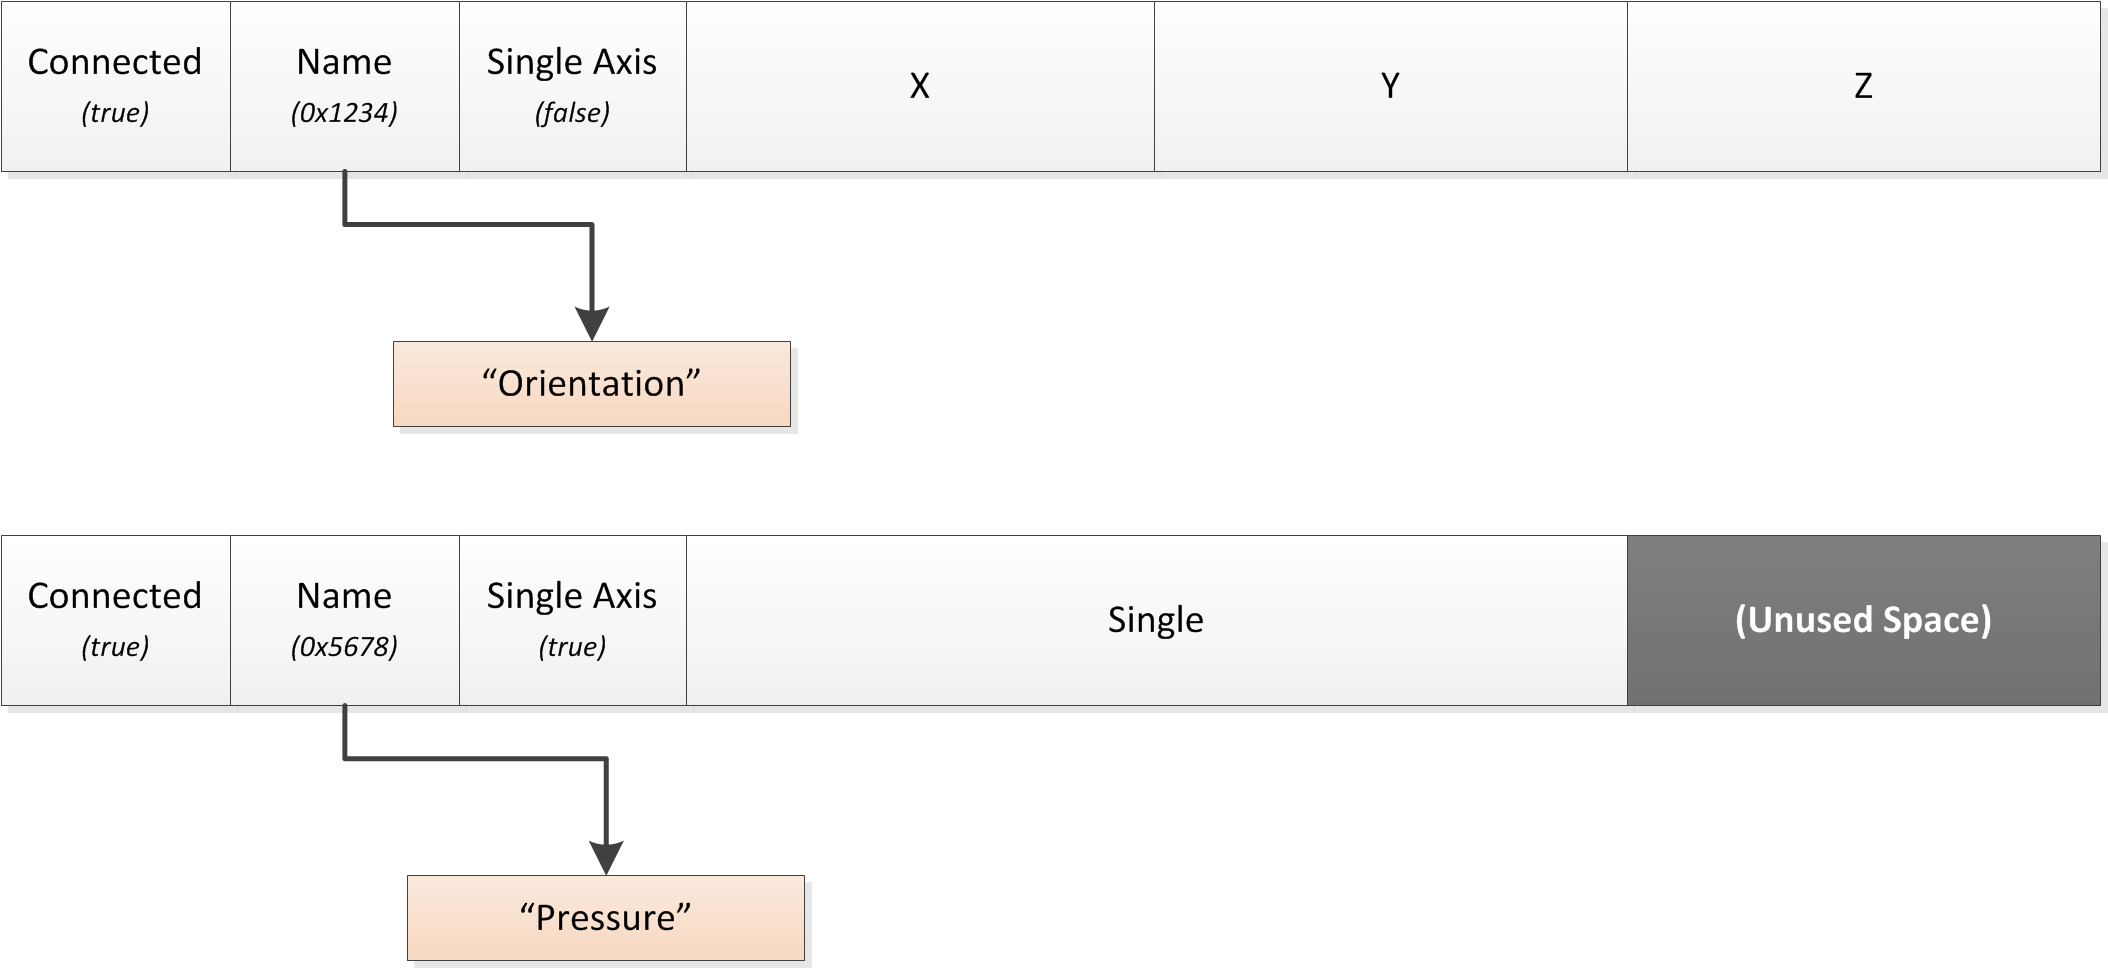
\includegraphics[width=130mm]{SensorPlatformEntry.png}
	\rule{35em}{0.5pt}
	\caption[Sensor Platform Entry Structure Diagram]{Diagram showing the layout of the Sensor Platform Entry structure in memory for triple axis (\textit{top}) and single axis (\textit{bottom}) sensors.}
	\label{fig:sensorentry}
\end{figure}

\FloatBarrier
\subsubsection{Individual Sensor Drivers}

Each individual sensor connected to the board requires a custom sensor driver, specific to that make and model of sensor IC. Unique to each sensor is the sequence required to set up the sensor to a known set of default configuration parameters (see Table \ref{tab:sensorconfig}), as well as the exact command set, address of the I\superscript{2}C bus, and optional use of control/interrupt GPIO lines used in the sensor's operation.

\begin{table}[tbph]
	\vspace{1em}
	\begin{center}
		\begin{tabular}{ | l | l | l | l | }
			\hline
			\textbf{Sensor}	& \textbf{Type}	& \textbf{Address} & \textbf{Settings} \\ \hline

			AK8975 & Direction & 0x0C & N/A \\ \hline
			BMA150 & Acceleration & 0x38 & \vtop{\hbox{\strut 25Hz bandwidth,} \hbox{\strut +/-2g range,} \hbox{\strut Interrupt line enabled}} \\ \hline
			BMP085 & Pressure & 0x77 & N/A \\ \hline
			ITG3200 & Orientation & 0x68 & \vtop{\hbox{\strut 100Hz at a 1KHz internal sampling rate,} \hbox{\strut Low Pass Filter to use 20Hz bandwidth,} \hbox{\strut Gyroscope X axis PLL as the clock source,} \hbox{\strut Interrupt line enabled}} \\ \hline
			ITG3200 & Temperature & 0x68 & N/A \textit{(Virtual Sensor)} \\ \hline
		\end{tabular}
		\caption[Sensor Configuration]{Table showing the sensors used and their configuration properties.}
		\label{tab:sensorconfig}
	\end{center}
\end{table}

To ensure the interface into each individual sensor driver was as uniform as possible, the exact implementation details was hidden from external modules, with each driver exposing just two functions; an \lstinline{Init()} function to initialize the sensor, and an \lstinline{Update()} function to pull the latest values from the sensor if it has completed a conversion. To prevent slow sensors from introducing unnecessary lag into the system, the update functions would abort if the next conversion was not ready at the point in time that the function was called, and the sensor entry structure would retain the previously retrieved sensor value. Each time a completed sensor data conversion was read from the sensor, a new conversion was started asynchronously.

\FloatBarrier
\subsection{Third Party Modules}

While every effort was made to ensure that as much code as possible for the project was written from scratch, some allowances had to be made for third party libraries. Such libraries were used in places where the complexity of the module would hinder the project if a new implementation had to be implemented from scratch within the project's time frame.

\FloatBarrier
\subsubsection{LUFA}

A crucial part of the project was the ability to communicate with USB devices; the AVR's USB interface was to be used for both configuration and control of the robot, via a variety of USB devices. A full USB stack is a rather complicated affair; generally it takes an entire team of programmers working together and ample debugging time to produce a functional stack. Because of the short time frame of the project, an existing stack was chosen instead.

The selected stack was LUFA, the \textit{Lightweight USB Framework for AVR devices}. This stack, a personal side-project of the author, offers a rich device support in both USB host and device modes. The library contains many inbuilt drivers for the various classes of USB devices, some of which were used in the project for the HID joystick control and Mass Storage configuration and sensor logging.

For the robot firmware, LUFA version 20111009 was used.

\FloatBarrier
\subsubsection{FatFS}

To read and write files onto an attached Mass Storage USB device, it was necessary to add a filesystem driver into the system. Using a standard filesystem allowed the firmware to maintain compatibility with files stored onto the disk using other devices. As the de-facto standard for embedded system filesystem is Microsoft's FAT (due to its relative simplicity when compared to more modern filesystems) a FAT compatible filesystem driver was selected for the project.

The third-party FATFs library was chosen for this task, as it offers a free, tested, portable and light-weight C implementation of the FAT filesystem standard. The FATFs library is compatible with most variants of the FAT standard (including FAT16 and FAT32) making it an ideal choice for the project. Linking the FATFs library's read and write callback functions to the LUFA USB library's Mass Storage class driver section functions proved to be much easier than anticipated (see Listing \ref{lst:fatfsshim}).

\lstinputlisting[float=tbph,caption={FATFs code to connect the library to the LUFA Mass Storage class driver.},label={lst:fatfsshim}]{./Figures/FATFsShim.c}

\FloatBarrier
\subsection{USB Management}

In order to support the various types of USB devices needed by the robot firmware, a collection of USB class-specific management layers were written. These layers, sitting in parallel on top of the LUFA USB stack, provide the routines necessary to manage each type of supported USB device.

While the LUFA USB stack provides support for several of these classes of USB devices internally, additional code was required to wrap the existing USB class driver, to extend the provided functionality and interface the driver with the rest of the system.

\FloatBarrier
\subsubsection{Bluetooth Adapters}

The LUFA stack version used in the project did not contain a ready-made internal driver for USB Bluetooth adapters. A suitable driver was thus created specifically for the project using the USB transport specification outlined in the Bluetooth 2.1 specification document. In order to support all possible Bluetooth adapters from all silicon vendors, the driver was written to match generically on the defined \texttt{class}, \texttt{subclass} and \texttt{protocol} Device Descriptor values of \texttt{0xE0}, \texttt{0x01} and \texttt{0x01} respectively, as set by the Bluetooth specification for conformant Bluetooth adapters. By matching against these values instead of a particular Vendor ID and Product ID, the driver was able to support all devices conforming to the Bluetooth standard's USB transport interface specification without additional modifications being required.

During the enumeration process of an inserted USB device, the main function calls the module's \lstinline{BluetoothAdapter_ConfigurePipes()} function to attempt to bind it to the inserted USB device. The module first validates the device descriptor to ensure the inserted device is reportedly a Bluetooth adapter. Next, the pipe configuration routine attempts to configure the USB controller's logical data pipes so that the \textit{Data In}, \textit{Data Out} and \textit{Event In} pipes are correctly connected to their matching logical endpoints within the adapter. If the driver is unable to bind to the device for any reason, the enumeration process is aborted for the Bluetooth transport driver.

Periodically, the main firmware loop will call the Bluetooth transport driver's \\ \lstinline{BluetoothAdapter_USBTask()} service task if the transport driver is currently active. This service task is responsible for checking the logical data pipes for new data, and (if data is available) reading in the data packet before dispatching it to the Bluetooth stack. A \lstinline{CALLBACK_Bluetooth_SendPacket()} callback function from the Bluetooth stack takes care of sending packets generated from the Bluetooth stack to the Bluetooth adapter.

\FloatBarrier
\subsubsection{HID Devices}

For local diagnostics of the system before the Bluetooth stack was completed, a local Human Interface Device (HID) driver was implemented into the firmware. This driver builds on top of the HID class driver included in the LUFA distribution used, and binds supported HID devices (such as game controllers) to the robot's physical functions. Using this driver, a USB joystick or game controller can be inserted into the robot and used to control the motors, headlights and horn.

As most HID devices carry a unique physical and logical report layout, it is important to include a mechanism to correctly bind the appropriate buttons on the attached device to the correct logical function. Two seemingly identical USB joysticks can output very different report data structures to the host, requiring the use of a \textit{HID Descriptor Report Parser} to correctly parse the reports into a standard format. The HID Report Parser included in the LUFA USB stack was used for this purpose, and linked into the rest of the system. This allows the robot to maintain compatibility with virtually all HID devices containing an appropriate number of buttons.

\FloatBarrier
\subsubsection{Mass Storage Devices}

As a means of system configuration and monitoring, a Mass Storage Device (MSD) driver was also added into the device firmware. This proved useful for both fault-finding and data logging, as data produced by the firmware could be stored onto an inserted USB flash drive. During the initial firmware development, this functionality was used to store logs of the on-board sensor outputs, to ensure the correctness of the sensor platform before the completion of the wireless serial port functionality. At a later stage, this mode was extended so that it could be used to configure the target remote Bluetooth Device Address used in the robot's Bluetooth Mode when a remote connection was initiated by the user.

To be able to read and write files on an attached USB flash disk drive, the FATFs library was linked to the LUFA Mass Storage class driver. This abstracted out the physical medium, giving a higher level file-centric view of the attached storage medium, as opposed to the direct physical sectors.

When a disk is inserted, the firmware will first attempt to open an existing file called \texttt{SENSLOG.CSV} on the disk, for sensor logging in CSV format (see Listing \ref{lst:logfileparse}). If such a file does not exist, a new one is created and the sensor log header (constructed by the Sensor Platform module) is written to the start of the new file.

\lstinputlisting[float=tbph,caption={Mass Storage manager code to open and write to a file on an attached USB flash disk using the FATFs library.},label={lst:logfileparse}]{./Figures/LogFileParsing.c}

Additionally, the firmware will attempt to open and process a second file on the attached storage disk named \texttt{REMADDR.TXT}, which holds the Bluetooth device address of the remote Bluetooth device the robot should attempt a connection to upon demand. This file is expected to contain an address of the format \texttt{XX:XX:XX:XX:XX:XX}, containing the six consecutive octets of the remote device's address, in hexadecimal format. This address is then stored into the robot's non-volatile EEPROM memory for later use when a Bluetooth adapter is subsequently inserted. If no such file exists on the attached disk, one is created and the currently stored remote device address written to it.

\FloatBarrier
\subsection{Bluetooth Management Layer}

Connecting the project's Bluetooth Stack to the rest of the robot firmware was the Bluetooth Management layer, responsible for providing the appropriate callback function implementations required by the stack. These callback functions are fired by the Bluetooth stack in response to defined events, such as connection requests, channel establishment and packet reception.

A secondary duty performed by the management software layer is the dispatch of events and data to and from the various Bluetooth services. These services, such as RFCOMM, SDP and HID, are optional in all implementations, and thus require manual integration into each project on top of the base Bluetooth stack if desired. These services must be linked to the various Bluetooth stack callback events so that they may function correctly (see Listing \ref{lst:btdatacallback}).

\lstinputlisting[float=tbph,caption={Bluetooth Stack event callback example, dispatching received packets to the integrated Bluetooth services.},label={lst:btdatacallback}]{./Figures/BTStackDataCallback.c}

In some cases, a Bluetooth enabled application may perform specific filtering on incoming connection and channel requests; an embedded device may be programmed to reject all but one specific remote device, or only accept specific channel protocols. However, as the \textit{ExplorerBot} was designed to be controlled publically via any supported Bluetooth enabled device, no such filtering was performed in the request callback routines. All HCI connection and L2CAP channel event callbacks were implemented, however, to display their relevant event data onto the robot's LCD display for debugging purposes.

Inside this management layer, the RFCOMM service channel open and close events were hooked, so that the opened RFCOMM channel handles could be captured. This captured handle is then stored temporarily by the robot firmware and used for later streaming of the sensor data. As only one connection handle is stored by the device at any one time for this purpose, a limitation of the system is imposed; only one wireless serial port can receive sensor data at the one time.

The HID service callback for packet reception was also hooked in this layer, and implemented to process incoming HID reports from Bluetooth devices. These processed reports---from game controllers, mobile phones, or other HID compliant devices---were then fed back into the main firmware module to control the robot's motors, headlights and horn hardware.